\documentclass[UTF8,a4paper,11pt]{ctexart}

% 本稿采用“校赛内部复核版”样式。题面未提供官方投稿模板，故不把本版式
% 宣称为高教社杯或校赛的官方格式；提交前需按主办方通知重新锁定格式。
\usepackage[a4paper,top=2.15cm,bottom=2.15cm,left=2.25cm,right=2.25cm]{geometry}
\usepackage{amsmath,amssymb,bm}
\usepackage{booktabs,tabularx,array,multirow,threeparttable}
\usepackage{graphicx,float}
\usepackage{xcolor}
\usepackage{enumitem}
\usepackage{listings}
\usepackage{hyperref}
\usepackage{caption}
\usepackage{fancyhdr}

% 支持从仓库根目录或 paper/ 目录调用编译器。
\graphicspath{{paper/figures/}{figures/}}
\definecolor{ink}{HTML}{203238}
\definecolor{jade}{HTML}{167C80}
\definecolor{rust}{HTML}{A44435}
\definecolor{papergray}{HTML}{F4F7F6}
\hypersetup{colorlinks=true,linkcolor=jade,urlcolor=jade,citecolor=jade}
\setlength{\parindent}{2em}
\setlength{\parskip}{0.25em}
\linespread{1.12}
\renewcommand{\arraystretch}{1.18}
\newcolumntype{Y}{>{\raggedright\arraybackslash}X}
\newcommand{\E}{\mathbb E}
\newcommand{\R}{\mathbb R}
\newcommand{\prob}{\mathbb P}
\newcommand{\code}[1]{\texttt{\detokenize{#1}}}
\DeclareMathOperator{\logit}{logit}
\DeclareMathOperator{\argmin}{arg\,min}
\DeclareMathOperator{\argmax}{arg\,max}

\pagestyle{fancy}
\fancyhf{}
\fancyhead[C]{\small 电信客户流失分析与挽留策略\quad\textbar\quad 校赛内部复核版}
\fancyfoot[C]{\thepage}
\setlength{\headheight}{14pt}

\title{\vspace{-1.0cm}\textbf{电信客户流失分析与挽留策略}\\[2mm]
  \large——基于可解释风险评分、经济阈值与压力情景的完整决策链}
\author{数学建模校赛 B 题\quad（匿名内部复核稿）}
\date{\today}

\begin{document}
\maketitle
\begin{abstract}
针对电信客户流失识别与挽留资源分配问题，本文将“描述高风险群体—输出个体风险—计算干预边界—应对外部冲击”组织为一条可复核的决策链。对附件中的 7043 条客户记录进行编码、缺失和重复审计后，样本流失率为 26.54\%。首先用列联表检验和修正 Cramér's V 识别关联因素，再以参考类别编码的 Logistic 回归给出可解释概率，并以五折 out-of-fold（OOF）预测隔离策略评估。模型 OOF ROC-AUC 为 0.8450，留出集 ROC-AUC 为 0.8422；月付合同、光纤服务、电子支票和短在网时长构成的交叉群体（\(n=440\)）观测流失率达到 75.45\%。

题目给定的单次挽留成本、历史成功率和流失损失分别为 150 元、0.35 和 2000 元，因此期望净收益判据为 \(p q L-C\geq0\)，概率阈值为 0.2143。按 OOF 风险实施阈值策略，选择 3286 人，期望净收益为 630184.63 元，高于全员干预的 253276.19 元。针对竞争对手降价、宏观下行和复合压力，本文以明确标注的 log-odds 扰动进行压力测试；复合压力下预测流失率为 33.89\%，稳健正收益集合的逐人净收益下界之和为 506335.09 元。由于数据是横截面且没有干预标签，文中所有风险关系均不解释为因果 uplift，外部冲击参数也不解释为已估计的价格弹性。
\end{abstract}

\noindent\textbf{关键词：}客户流失；Logistic 回归；OOF 预测；经济阈值；稳健挽留；压力测试

\section{问题重述与总体路线}\label{sec:problem}

题面要求围绕客户画像完成四项工作：\textbf{Q1} 找出更容易流失的客户群体并分析因素关系；\textbf{Q2} 综合合同、在网时长、月费用和增值服务，给出客户流失判定方法；\textbf{Q3} 在每次挽留成本 150 元、历史成功率 35\%、单个流失损失约 2000 元的条件下设计策略；\textbf{Q4} 在竞争价格和宏观环境变化下检验策略稳健性并给出动态调整方法。本文不把四问拆成互不相连的模型，而是使用图~\ref{fig:route} 所示的接口：Q1 的群体证据解释 Q2 的特征，Q2 输出的 OOF 概率进入 Q3 的经济判据，Q4 对同一概率的 logit 进行可审计扰动。

\begin{figure}[H]
  \centering
  \fbox{\parbox{0.92\linewidth}{\centering\small
  数据审计 \(\longrightarrow\) Q1 关联与群体\(\longrightarrow\) Q2 风险概率\\[1mm]
  \hfill\(\searrow\)\quad\quad\quad\quad\quad\quad\quad\quad\(\swarrow\)\\[-1mm]
  \hfill Q3 经济阈值与容量分配\quad Q4 压力情景与稳健调整}}
  \caption{四个小问之间的模型接口；箭头表示输出量的复用，不表示因果关系。}
  \label{fig:route}
\end{figure}

\subsection{题面范围与格式口径}
本稿使用用户提供的《校赛 B 题》题面和附件，竞赛版本记为“2026 华中师范大学数学建模竞赛、B 题”。题面未随附件提供可核验的官方论文模板、页数和匿名细则，因此本文的页面参数只服务于数学与结果复核，官方格式状态为\emph{待主办方确认}。任何投稿前版本都应把本稿内容迁移到当届官方模板，并重新进行渲染审计。

\section{数据审计、变量与假设}\label{sec:data}

\subsection{数据结构与清洗}
附件共有 21 列：客户编码、性别、老年标记、伴侣/家属、在网时长、电话与线路、互联网及五类增值服务、合同与支付、月费用、总费用和是否流失。客户编码只用于本地风险明细，不进入本文的统计汇总。表~\ref{tab:quality} 给出可复核的质量摘要。

\begin{table}[H]
\centering
\caption{附件数据质量与目标分布}
\label{tab:quality}
\begin{tabular}{@{}llr@{}}
\toprule
项目 & 口径 & 数值\\
\midrule
记录数 & 行（不含表头） & 7043\\
字段数 & 列 & 21\\
编码 & 自动探测结果 & \code{gb18030}\\
重复记录 & 完全重复行 & 0\\
重复客户编码 & ID 重复数 & 0\\
流失/未流失 & 目标计数 & 1869 / 5174\\
总体流失率 & \(1869/7043\) & 26.54\%\\
总费用空值 & 原始空字符串 & 11\\
空值处理 & 在网时长为 0 的空总费用 & 置为 0\\
\bottomrule
\end{tabular}
\begin{tablenotes}
\footnotesize\item 注：11 条空总费用均对应在网时长 0 个月；没有剩余总费用缺失需要用中位数填补。数值均来自本地求解器的聚合输出。
\end{tablenotes}
\end{table}

记第 \(i\) 个客户的流失标签为 \(Y_i\in\{0,1\}\)，其中 1 表示“是”。对于总费用，清洗规则写成
\begin{equation}
T_i^*=\begin{cases}
0, & T_i\text{ 为空且 }U_i=0,\\
T_i, & \text{其他可解析数值},
\end{cases}
\label{eq:data-clean}
\end{equation}
其中 \(U_i\) 是在网时长（月），\(T_i^*\) 的单位为元。该规则只修正由题面字段组合确定的结构性空值，不对未知缺失作无依据的插补。

\subsection{变量注册与可检验假设}
表~\ref{tab:symbols} 只列出后续公式中反复出现的符号；原始字段与模型字段的完整映射保存在求解器中。

\begin{table}[H]
\centering
\caption{主要符号、单位与来源}
\label{tab:symbols}
\begin{tabularx}{\linewidth}{@{}l l Y l@{}}
\toprule
符号 & 类型 & 含义 & 单位/粒度\\
\midrule
\(Y_i\) & 输入/响应 & 客户 \(i\) 是否流失 & 无量纲/客户\\
\(\boldsymbol{x}_i\) & 输入 & 合同、服务、费用等画像特征 & 混合/客户\\
\(p_i\) & 输出 & 客户流失的关联风险概率 & 无量纲/客户\\
\(C\) & 参数 & 一次挽留干预成本 & 元/客户\\
\(q\) & 参数 & 对将要流失客户的平均成功率 & 无量纲\\
\(L\) & 参数 & 一个流失客户的损失 & 元/客户\\
\(d_i\) & 决策 & 是否对客户 \(i\) 实施干预 & \(0/1\)/客户\\
\(\delta_i^{(s)}\) & 情景参数 & 情景 \(s\) 的 log-odds 扰动 & 无量纲/客户\\
\bottomrule
\end{tabularx}
\end{table}

为使结论可被攻击，本文采用以下假设，并在验证章节写明放松方式：
\begin{enumerate}[label=\textbf{A\arabic*}.,leftmargin=2.5em]
  \item 在同一观测截面内，字段定义和标签口径一致；若未来标签窗口改变，模型需重新训练。
  \item Logistic 模型只描述条件关联风险，不把系数解释为干预造成的变化；若需要个体化优惠效果，必须补充随机挽留实验。
  \item Q3 的 \(q=0.35\) 和 \(L=2000\) 是题面给定的期望参数；Q4 的 \(\delta\)、情景成功率和成本是压力假设，不能替代外部冲击数据。
  \item 由于附件没有时间、地区、竞争价格和宏观变量，Q4 只提供情景边界与调整规则，不声称识别动态弹性。
\end{enumerate}

\section{Q1：流失群体与因素关系}\label{sec:q1}

\subsection{列联表检验}
对每个类别字段 \(X_j\)，将其水平记为 \(a\)，观测频数为 \(n_{ay}\)，边际频数为 \(n_{a\cdot}\) 和 \(n_{\cdot y}\)。独立性假设下的期望频数为
\begin{equation}
e_{ay}=\frac{n_{a\cdot}n_{\cdot y}}{N},\qquad
\chi_j^2=\sum_{a}\sum_{y\in\{0,1\}}\frac{(n_{ay}-e_{ay})^2}{e_{ay}}.
\label{eq:q1-chi}
\end{equation}
为避免样本量很大时仅凭显著性排序，进一步报告修正 Cramér's V：
\begin{equation}
V_j=\sqrt{\frac{\max\left(0,\phi_j^2-\frac{(k_j-1)(r_j-1)}{N-1}\right)}{\min(k_j-1,r_j-1)}},
\qquad \phi_j^2=\frac{\chi_j^2}{N},
\label{eq:q1-cramers}
\end{equation}
其中 \(r_j\) 和 \(k_j\) 分别是列联表的行、列数。\(V_j\) 越大，表示该字段与标签的观测关联越强，但不包含时间顺序或干预识别。

\begin{table}[H]
\centering
\caption{类别字段与流失标签的关联强度（按 Cramér's V 降序）}
\label{tab:q1-association}
\begin{tabular}{@{}lrrrr@{}}
\toprule
字段 & 水平数 & \(\chi^2\) & \(p\) 值 & \(V\)\\
\midrule
合同类型 & 3 & 1184.60 & \(5.86\times10^{-258}\) & 0.410\\
在线安全 & 3 & 850.00 & \(2.66\times10^{-185}\) & 0.347\\
技术支持 & 3 & 828.20 & \(1.44\times10^{-180}\) & 0.343\\
互联网服务类型 & 3 & 732.31 & \(9.57\times10^{-160}\) & 0.322\\
支付方式 & 4 & 648.14 & \(3.68\times10^{-140}\) & 0.303\\
在线备份 & 3 & 601.81 & \(2.08\times10^{-131}\) & 0.292\\
设备保护 & 3 & 558.42 & \(5.51\times10^{-122}\) & 0.281\\
电影流媒体 & 3 & 375.66 & \(2.67\times10^{-82}\) & 0.230\\
性别 & 2 & 0.48 & 0.487 & 0.000\\
电话服务 & 2 & 0.92 & 0.339 & 0.000\\
\bottomrule
\end{tabular}
\begin{tablenotes}
\footnotesize\item 注：\(p\) 值仅用于独立性检验；不将统计显著性等同于业务重要性或因果性。完整 16 个类别字段表保存在 \code{paper/evidence/associations.csv}。
\end{tablenotes}
\end{table}

\subsection{群体流失率与交叉画像}
对群体 \(G\) 定义观测流失率
\begin{equation}
\widehat p(G)=\frac{\sum_{i=1}^{N}\mathbb{1}(i\in G)Y_i}{\sum_{i=1}^{N}\mathbb{1}(i\in G)}.
\label{eq:q1-group-rate}
\end{equation}
图~\ref{fig:groups} 展示合同、互联网、支付和在网时长四个维度；交叉群体的分母和流失率列于表~\ref{tab:intersections}。结果显示，月付合同、光纤服务、电子支票和短在网时长分别形成高风险信号；叠加后风险进一步集中。

\begin{figure}[H]
  \centering
  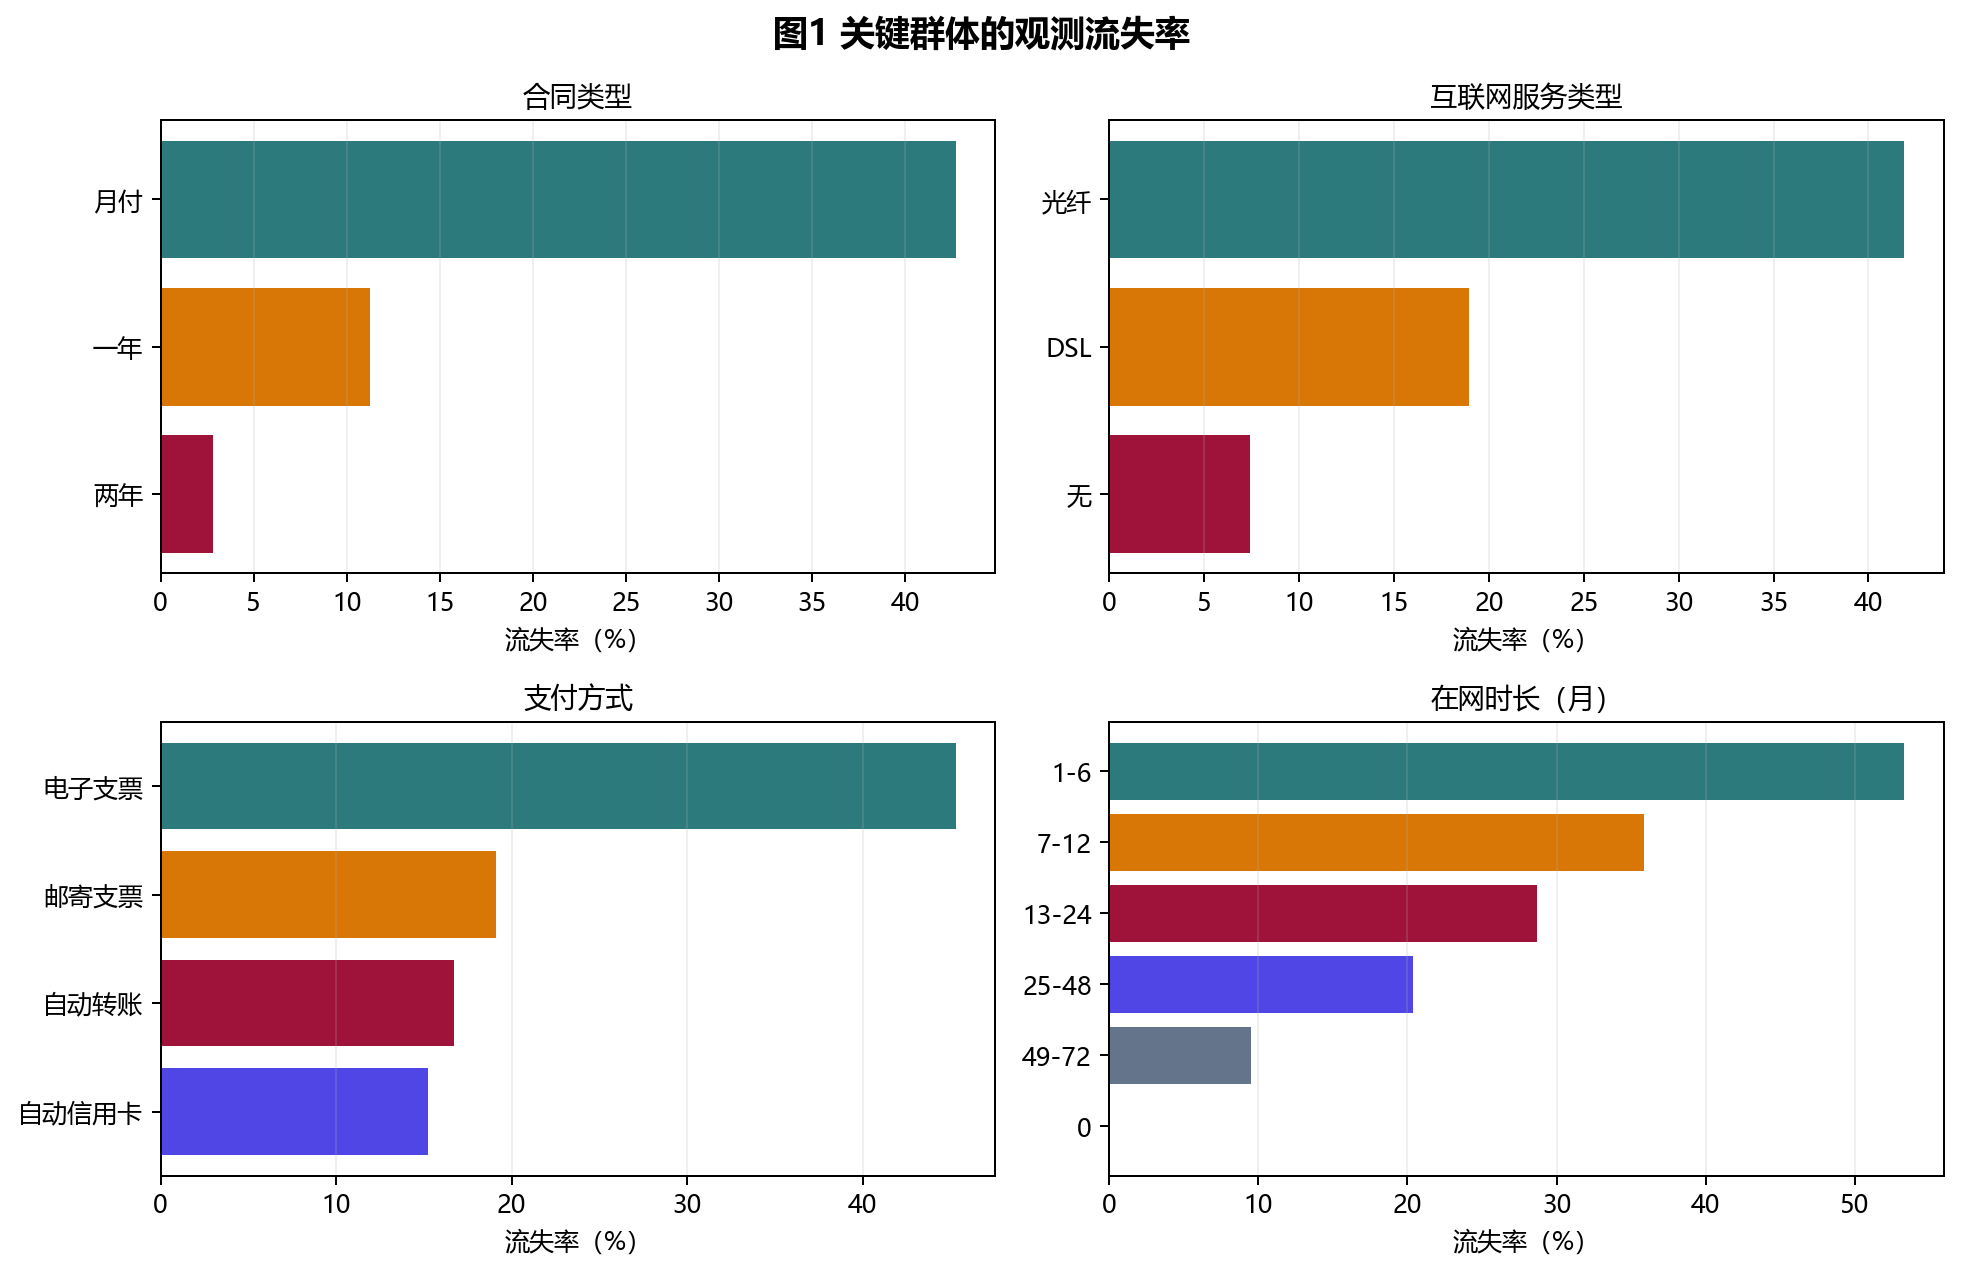
\includegraphics[width=0.93\linewidth]{fig_churn_groups.png}
  \caption{关键群体的观测流失率；每个柱子的分母为该群体客户数，不能单独推出干预效果。}
  \label{fig:groups}
\end{figure}

\begin{table}[H]
\centering
\caption{代表性交叉群体的观测流失率}
\label{tab:intersections}
\begin{tabular}{@{}lrr@{}}
\toprule
群体条件 & 样本数 & 流失率\\
\midrule
月付合同 & 3875 & 42.71\%\\
光纤服务 & 3096 & 41.89\%\\
电子支票 & 2365 & 45.29\%\\
在网不超过 6 个月 & 1481 & 52.94\%\\
月付 + 光纤 & 2128 & 54.61\%\\
月付 + 电子支票 & 1850 & 53.73\%\\
月付 + 光纤 + 电子支票 & 1307 & 60.37\%\\
月付 + 光纤 + 电子支票 + 在网不超过 6 个月 & 440 & 75.45\%\\
\bottomrule
\end{tabular}
\begin{tablenotes}
\footnotesize\item 注：这些是同一横截面中的分组描述；交叉条件可能共享同一潜在机制，不能将各差值相加解释为独立贡献。
\end{tablenotes}
\end{table}

因此，Q1 的可操作画像是“月付、短在网、光纤、电子支票、缺少安全/支持服务”的优先核查群体；性别和电话服务在本数据中几乎没有单变量区分度。该画像作为 Q2 的解释层与 Q3 的分层运营入口，而不是绕过概率模型的硬编码结论。

\section{Q2：可解释的流失判定方法}\label{sec:q2}

\subsection{参考编码的 Logistic 风险模型}
令数值变量集合为 \(\mathcal N=\{U,M,T^*\}\)，分别表示在网时长、月费用和清洗后的总费用；类别变量集合记为 \(\mathcal C\)。数值变量以训练折中位数填补后标准化，类别变量以训练折众数填补并对每个字段丢弃一个参考水平。模型的线性预测量和概率为
\begin{equation}
z_i=\beta_0+\sum_{j\in\mathcal N}\beta_j\frac{x_{ij}-\widetilde x_j}{s_j}
 +\sum_{j\in\mathcal C}\sum_{\ell\ne\ell_{j0}}\beta_{j\ell}\mathbb{1}(x_{ij}=\ell),
\qquad \widehat p_i=\sigma(z_i)=\frac{1}{1+e^{-z_i}}.
\label{eq:q2-logistic}
\end{equation}
丢弃参考水平后的系数是相对于 \(\ell_{j0}\) 的条件对数优势比；数值变量的优势比对应增加一个训练样本标准差。参数通过带 \(L_2\) 正则的对数损失估计：
\begin{equation}
\widehat{\bm\beta}=\argmin_{\bm\beta}\left\{-\sum_{i\in\mathcal T}\left[Y_i\log \widehat p_i+(1-Y_i)\log(1-\widehat p_i)\right]+\frac{\lambda}{2}\lVert\bm\beta\rVert_2^2\right\}.
\label{eq:q2-fit}
\end{equation}
式~\eqref{eq:q2-logistic} 的概率是判别排序工具。由于总费用、月费用和在网时长存在结构相关，单个系数只能作为条件关联方向，不能被改写成价格或服务变更的因果效应。

\subsection{隔离验证与模型选择}
采用固定随机种子 42 的分层五折交叉验证：每一折只用其余四折拟合预处理器和模型，再对留出折产生 OOF 概率；所有客户的 OOF 概率拼接后用于校准和 Q3 策略计算。最后再用全体样本拟合一个模型，生成本地运营风险明细。非线性的 HistGradientBoosting 只作为同字段基准，不因模型更复杂就自动替换可解释主模型。

\begin{table}[H]
\centering
\caption{风险模型的隔离验证指标}
\label{tab:q2-metrics}
\begin{tabular}{@{}lrrrrrr@{}}
\toprule
模型/数据 & ROC-AUC & AP & Brier & Log loss & 精确率 & 召回率\\
\midrule
Logistic，留出集 & 0.8422 & 0.6349 & 0.1380 & 0.4203 & 0.6593 & 0.5588\\
梯度提升，留出集 & 0.8380 & 0.6462 & 0.1385 & 0.4267 & 0.6575 & 0.5134\\
Logistic，五折 AUC 均值±标准差 & \multicolumn{5}{r}{0.8450 $\pm$ 0.0135}\\
Logistic，OOF & 0.8450 & 0.6539 & 0.1356 & 0.4174 & 0.6592 & 0.5527\\
\bottomrule
\end{tabular}
\begin{tablenotes}
\footnotesize\item 注：AP 为 average precision；精确率和召回率使用概率 0.5，仅用于报告，不是 Q3 的经济阈值。完整指标和折次保存在 \code{paper/evidence/model_metrics.json}。
\end{tablenotes}
\end{table}

图~\ref{fig:roc} 给出留出集 ROC 曲线。OOF 十分位校准中，最低到最高风险箱的平均预测概率分别约为 0.0053 和 0.7244，对应观测流失率约为 1.28\% 和 75.89\%，说明概率具有明显的风险分层能力，但仍需在新时间窗口上复校准。

\begin{figure}[H]
  \centering
  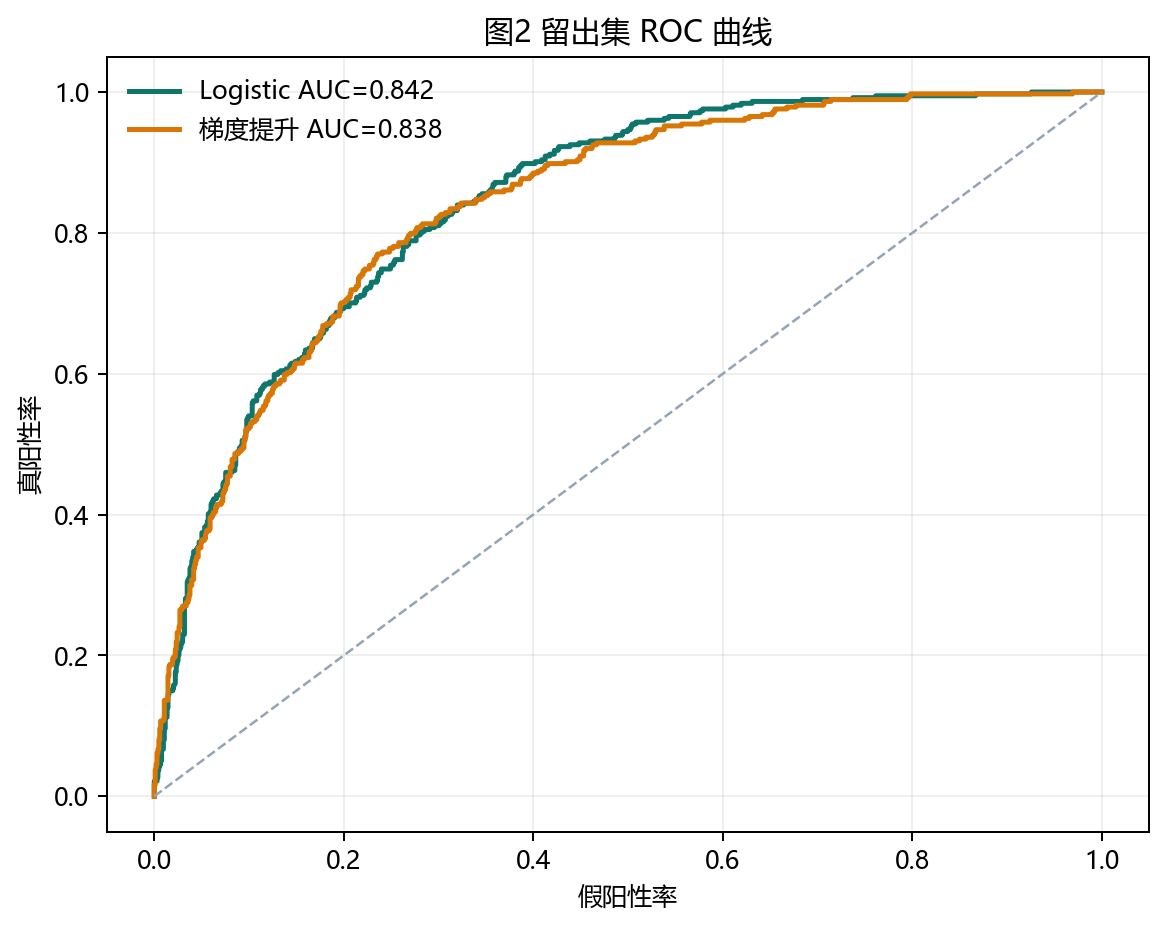
\includegraphics[width=0.70\linewidth]{fig_roc.png}
  \caption{留出集 ROC 曲线；曲线只衡量本横截面上的区分度，不是未来时间外推证明。}
  \label{fig:roc}
\end{figure}

\begin{figure}[H]
  \centering
  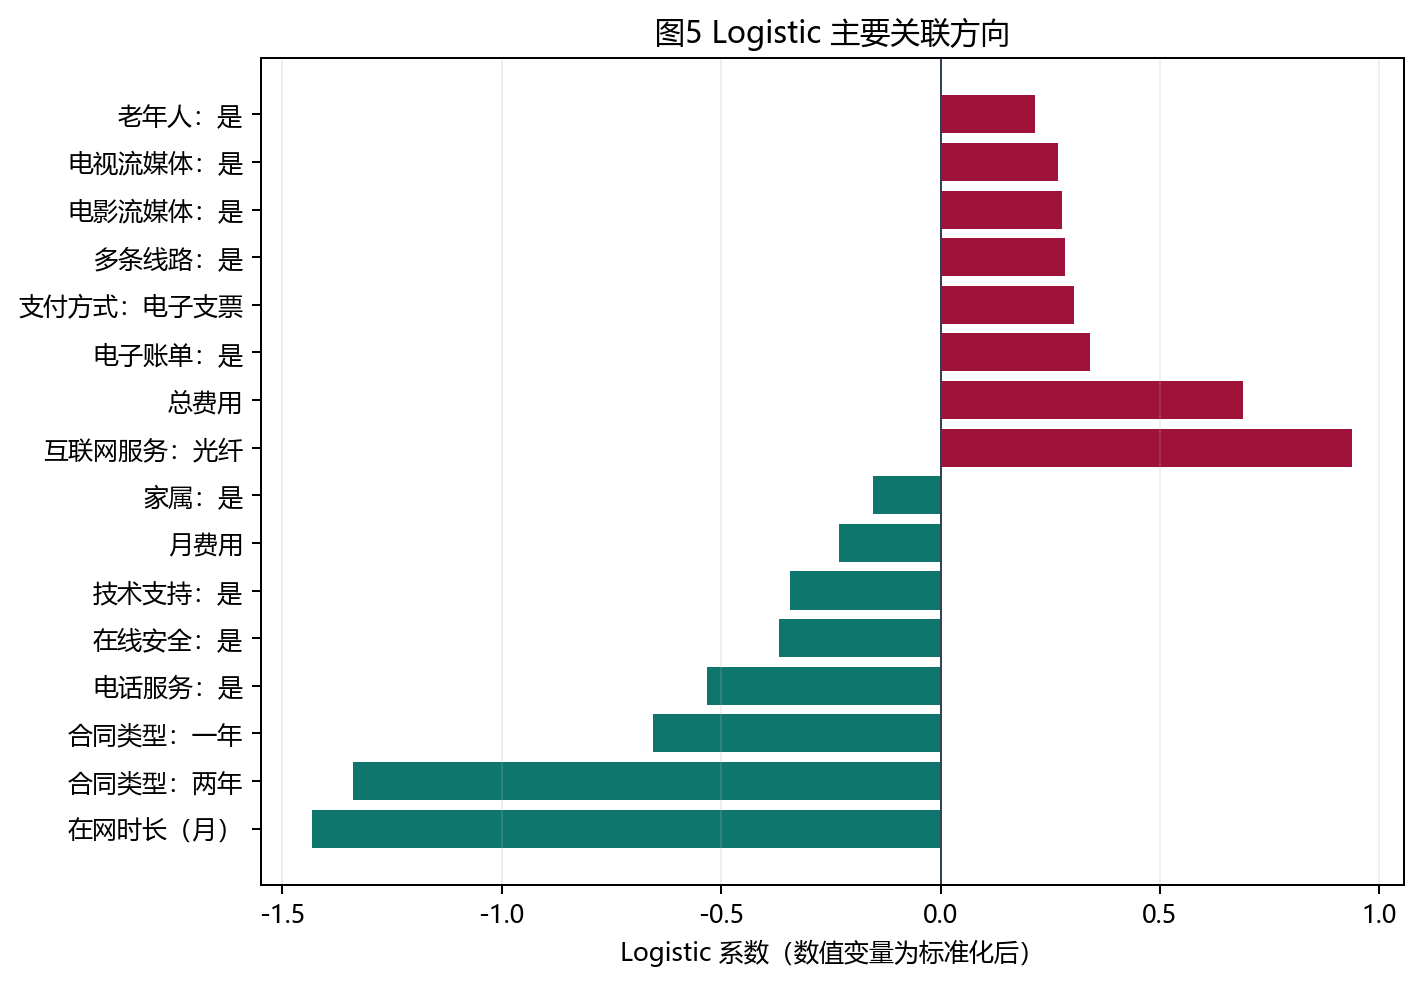
\includegraphics[width=0.86\linewidth]{fig_feature_effects.png}
  \caption{参考类别编码下的主要 Logistic 关联方向；数值变量已标准化，系数不代表因果效应。}
  \label{fig:effects}
\end{figure}

\subsection{判定规则与可解释输出}
给定客户画像后，先按式~\eqref{eq:q2-logistic} 得到 \(\widehat p_i\)，再按照 Q3 的经济门决定是否进入干预候选集。若只需要“高风险/低风险”标签，可以使用题目成本参数导出的阈值，而不把 0.5 当成普适标准。模型最终输出应至少包含概率、主要触发特征、参考水平和数据时间窗；若出现训练时未见的类别，保留安全的未知水平编码并标记需复核。

\section{Q3：挽留策略与资源分配}\label{sec:q3}

\subsection{期望净收益判据}
对客户 \(i\) 实施一次干预的成本为 \(C\)。若客户在不干预时流失的概率为 \(p_i\)，对“将要流失客户”的平均挽留成功率为 \(q\)，每个流失客户损失为 \(L\)，则期望避免损失为 \(p_iqL\)，单客期望净收益为
\begin{equation}
g_i=p_iqL-C.
\label{eq:q3-person-net}
\end{equation}
对候选集合 \(S\) 的总期望净收益为
\begin{equation}
B(S)=\sum_{i\in S}g_i
 =\sum_{i\in S}(p_iqL-C),
\qquad d_i=\mathbb{1}(i\in S).
\label{eq:q3-objective}
\end{equation}
当没有容量约束时，逐人目标可分离，最优集合为 \(S^*=\{i:g_i\geq0\}\)，即
\begin{equation}
\tau=\frac{C}{qL}=\frac{150}{0.35\times2000}=0.2142857,
\qquad S^*=\{i:\widehat p_i\geq\tau\}.
\label{eq:q3-threshold}
\end{equation}
当每天只能处理 \(K\) 人时，将 \(g_i\) 从大到小排序，取前 \(K\) 人。交换论证很直接：若集合中有较小的 \(g_a\)，集合外有较大的 \(g_b\)，用 \(b\) 替换 \(a\) 会使目标增加 \(g_b-g_a>0\)，所以排序截断是容量约束下的最优选择。

\subsection{策略比较}
表~\ref{tab:q3-policy} 使用同一组 OOF 概率和题面参数比较全员、经济阈值及固定比例策略。\(\widehat p_i\) 只来自不包含该客户的训练折，避免直接用训练内拟合概率夸大收益。

\begin{table}[H]
\centering
\caption{不同挽留策略的期望收益（OOF 概率）}
\label{tab:q3-policy}
\scriptsize
\setlength{\tabcolsep}{3.2pt}
\begin{tabular}{@{}lrrrrr@{}}
\toprule
策略 & 选择人数 & 覆盖率 & 选中组观测流失率 & 期望避免损失/元 & 期望净收益/元\\
\midrule
不干预 & 0 & 0.00\% & -- & 0.00 & 0.00\\
全员干预 & 7043 & 100.00\% & 26.54\% & 1309726.19 & 253276.19\\
经济阈值 \(p\ge0.2143\) & 3286 & 46.66\% & 48.23\% & 1123084.63 & 630184.63\\
风险排序前 1\% & 70 & 0.99\% & 85.71\% & 39711.87 & 29211.87\\
风险排序前 5\% & 352 & 5.00\% & 81.25\% & 187597.37 & 134797.37\\
风险排序前 10\% & 704 & 10.00\% & 75.99\% & 357051.44 & 251451.44\\
风险排序前 20\% & 1408 & 20.00\% & 67.40\% & 649322.14 & 438122.14\\
\bottomrule
\end{tabular}
\begin{tablenotes}
\footnotesize\item 注：期望避免损失使用 \(\sum_{i\in S}\widehat p_i qL\)，干预成本为选择人数乘 150 元；选中组观测流失率仅作独立的描述性校验，不等于挽留后的实际成功率。
\end{tablenotes}
\end{table}

图~\ref{fig:policy} 表明，按经济阈值筛出的集合比全员干预保留了更多净收益。实际运营可采用“阈值筛选—容量排序—分层话术”的两级策略：先排除 \(g_i<0\) 的低收益客户，再在剩余客户中按风险和服务成本排序；对 Q1 的交叉高风险群体优先核查合同解释、光纤服务体验和电子支票支付摩擦，而不是对所有人发送同一优惠。

\begin{figure}[H]
  \centering
  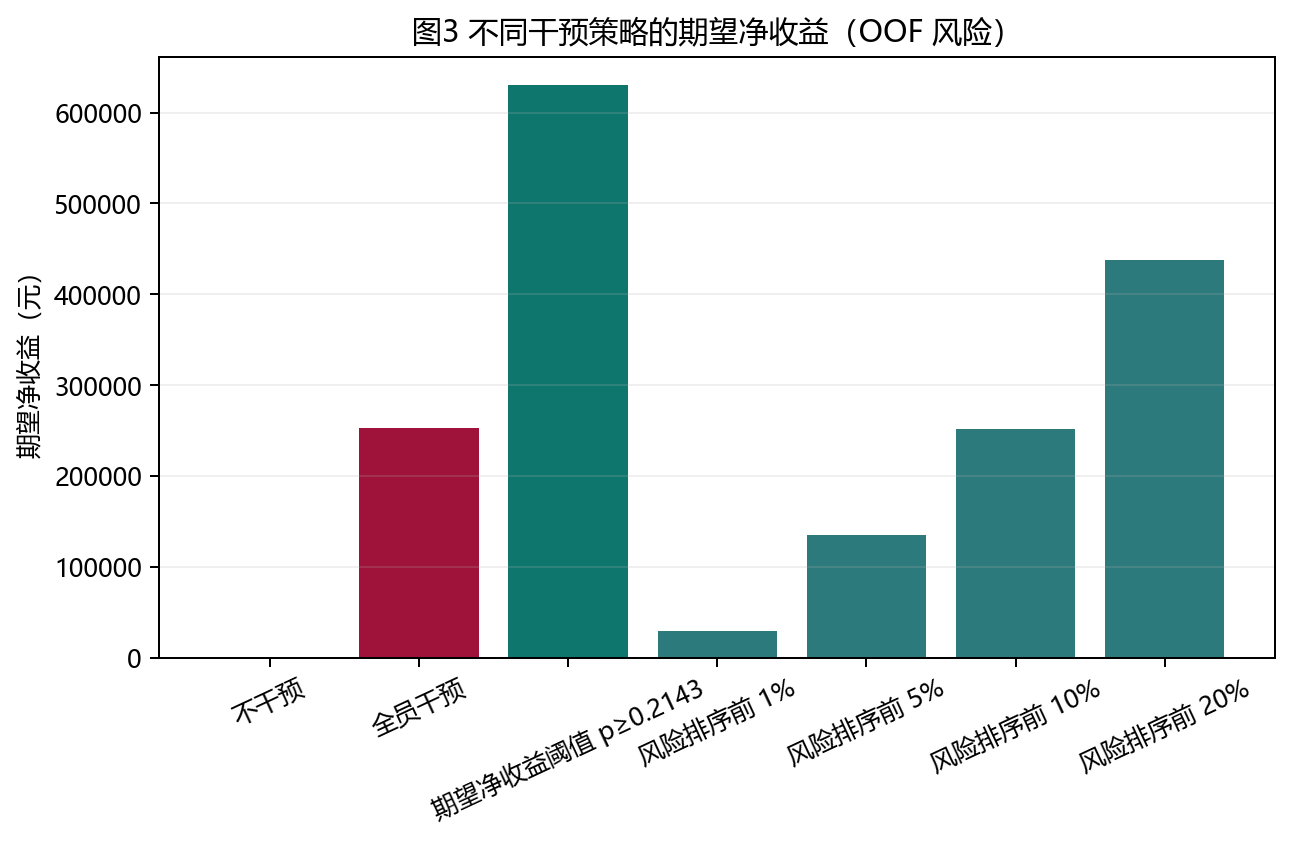
\includegraphics[width=0.86\linewidth]{fig_policy.png}
  \caption{不同干预策略的期望净收益；金额为题面参数下的模型期望，不是已实现现金流。}
  \label{fig:policy}
\end{figure}

\subsection{参数敏感性}
式~\eqref{eq:q3-threshold} 说明成功率下降或单客损失下降都会提高阈值。令 \(q\) 取 0.25、0.35、0.45，\(L\) 取 1500、2000、2500 元，部分结果见表~\ref{tab:q3-sensitivity}。所有组合仍使用同一 OOF 概率，变化来自经济口径而非重新训练模型。

\begin{table}[H]
\centering
\caption{挽留成功率与流失损失的敏感性（代表组合）}
\label{tab:q3-sensitivity}
\begin{tabular}{@{}rrrrr@{}}
\toprule
\(q\) & \(L\)/元 & 阈值 \(C/(qL)\) & 选择人数 & 期望净收益/元\\
\midrule
0.25 & 1500 & 0.4000 & 2103 & 153341.36\\
0.25 & 2000 & 0.3000 & 2658 & 322936.25\\
0.35 & 2000 & 0.2143 & 3286 & 630184.63\\
0.45 & 2000 & 0.1667 & 3773 & 961295.39\\
0.45 & 2500 & 0.1333 & 4047 & 1348110.77\\
\bottomrule
\end{tabular}
\end{table}

\section{Q4：外部冲击下的稳健策略}\label{sec:q4}

\subsection{压力情景的构造}
附件没有竞争价格、宏观指标或时间序列，不能从数据估计外部冲击系数。为回答“如何调整”而不伪造因果证据，本文把冲击写成透明的 log-odds 压力参数：
\begin{equation}
p_i^{(s)}=\sigma\!\left(\logit(\widehat p_i)+\delta_i^{(s)}\right),
\qquad
\logit(p)=\log\frac{p}{1-p}.
\label{eq:q4-shift}
\end{equation}
竞争降价情景对月付、一年、两年合同分别加入 0.35、0.15、0.05；宏观下行情景对全体加入 0.20，在网时长不足 12 个月者再加入 0.05。情景同时改变成功率和干预成本，以检验策略而非只抬高概率。

\begin{table}[H]
\centering
\caption{外部冲击情景与结果}
\label{tab:q4-scenarios}
\begin{tabular}{@{}lrrrrr@{}}
\toprule
情景 & 平均 logit 扰动 & 成功率 & 成本/元 & 预测流失率 & 正收益人数\\
\midrule
基准 & 0.000 & 0.35 & 150 & 26.57\% & 3286\\
竞争对手降价 & 0.236 & 0.33 & 150 & 30.79\% & 3624\\
宏观下行 & 0.215 & 0.30 & 165 & 29.63\% & 3140\\
复合压力 & 0.451 & 0.28 & 180 & 33.89\% & 3252\\
\bottomrule
\end{tabular}
\begin{tablenotes}
\footnotesize\item 注：扰动、成功率和成本是压力假设；“正收益人数”表示在该假设下按 \(p_i^{(s)}q_sL-C_s>0\) 的人数，不是实际接受优惠人数。
\end{tablenotes}
\end{table}

\begin{figure}[H]
  \centering
  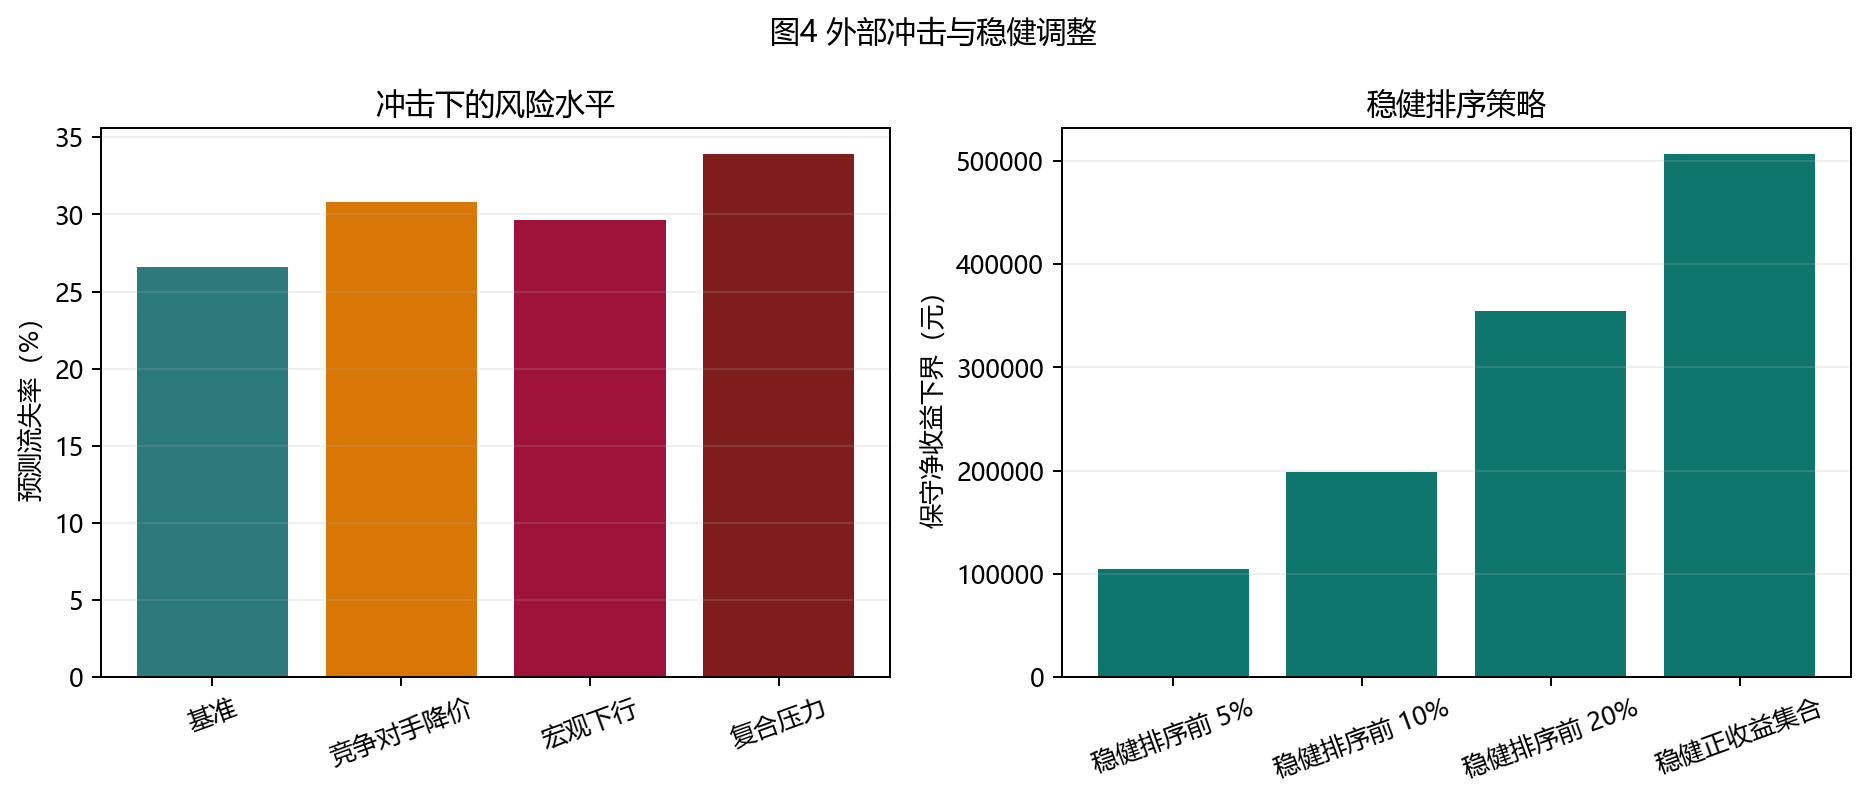
\includegraphics[width=0.90\linewidth]{fig_scenarios.png}
  \caption{外部冲击与稳健排序；左图为风险水平，右图为逐人最坏净收益下界的累加。}
  \label{fig:scenarios}
\end{figure}

\subsection{稳健目标与动态调整规则}
令情景集合为 \(\mathcal S\)，情景 \(s\) 下的单客净收益为 \(g_i^{(s)}=p_i^{(s)}q_sL-C_s\)。保守地定义逐人最坏得分
\begin{equation}
r_i=\min_{s\in\mathcal S}g_i^{(s)},
\qquad S_R=\{i:r_i>0\}.
\label{eq:q4-robust}
\end{equation}
在各客户成本已包含于 \(g_i^{(s)}\) 的前提下，选择 \(S_R\) 可保证每个入选客户在所有压力情景下仍有正的逐人期望净收益。表~\ref{tab:q4-robust} 给出风险排序和稳健正收益集合；“下界”是 \(\sum_{i\in S}\min_s g_i^{(s)}\)，不是对未来现金流的置信区间。

\begin{table}[H]
\centering
\caption{稳健策略的保守收益下界}
\label{tab:q4-robust}
\begin{tabular}{@{}lrrr@{}}
\toprule
策略 & 选择人数 & 覆盖率 & 逐人最坏净收益下界之和/元\\
\midrule
稳健排序前 5\% & 352 & 5.00\% & 104595.98\\
稳健排序前 10\% & 704 & 10.00\% & 198611.50\\
稳健排序前 20\% & 1408 & 20.00\% & 354597.05\\
稳健正收益集合 & 3122 & 44.33\% & 506335.09\\
\bottomrule
\end{tabular}
\end{table}

据此给出可落地的月度动态规则：
\begin{enumerate}[label=\textbf{D\arabic*}.,leftmargin=2.5em]
  \item 每个标签窗口重新计算数据漂移、校准曲线和合同分层流失率；若新窗口的校准误差或 AUC 超过预设门限，暂停自动扩大覆盖率。
  \item 根据竞争价格和宏观指标（补充采集后）估计或更新 \(\delta_i^{(s)}\)，同时重新审查 \(q_s,C_s,L\)；在证据不足时沿用压力上界而不输出“已估计弹性”。
  \item 先用 \(r_i>0\) 的稳健集合做保守投放；若容量有限，按 \(r_i\) 排序。对月付且在网不足 12 个月者设置人工复核，避免一次性高额优惠伤害长期价值。
  \item 用随机对照实验记录“是否触达、优惠内容、是否续留和成本”，逐步把题面平均成功率替换为分层的实验估计；在实验完成前不把相关模型升级为个体 uplift 模型。
\end{enumerate}

\section{验证、局限与推广}\label{sec:validation}

本文使用了四类互补检查：\(\text{(i)}\) 数据行列、重复和结构性缺失审计；\(\text{(ii)}\) 列联表与交叉群体的独立描述；\(\text{(iii)}\) 留出集、五折 AUC、OOF 校准和非线性基准；\(\text{(iv)}\) 经济参数敏感性与外部冲击压力测试。图~\ref{fig:effects} 的系数方向、表~\ref{tab:q3-policy} 的策略排序和表~\ref{tab:q4-robust} 的稳健下界均由同一求解入口生成，避免手工改写数字。

仍有以下边界：
\begin{enumerate}[label=\arabic*.,leftmargin=2.5em]
  \item 横截面数据不能证明“降价、电子支票或缺少支持服务导致流失”；只能支持观测关联和风险排序。
  \item OOF 验证随机分层而非按时间切分；部署到未来月份前必须补做时间外推回测，检查概念漂移。
  \item \(q=0.35\) 是全体平均成功率，未区分客户可挽留性；Q3 的收益是期望决策值，不是承诺的实际利润。
  \item Q4 的 logit 扰动是可解释的压力假设。没有竞争价格、宏观变量和外部时间序列时，不能把情景差异写成市场弹性估计。
  \item 总费用与在网时长、月费用存在结构相关，系数表不宜用于单独制定价格政策；业务解释应回到分层实验。
\end{enumerate}

若补充连续月份标签、触达记录、竞争价格、服务工单和地区信息，可将当前链条升级为时间切分的校准模型、分层 uplift 实验和带预算约束的多期优化；在此之前，本文的保守阈值和稳健集合是更适合上线试运行的接口。

\section{结论}\label{sec:conclusion}

本题的核心不是对所有客户套用同一个分类器，而是把数学判据与运营约束接起来。数据证据显示，合同期限、服务组合、支付方式和在网时长是主要风险分层线索；参考编码 Logistic 模型在 OOF 上达到 0.8450 的 ROC-AUC，并输出可解释概率。把题面经济参数代入 \(p q L-C\) 后，阈值 0.2143 将“是否干预”变为可复核不等式，OOF 评估下选择 3286 人的期望净收益约 63.02 万元。面对外部冲击，使用 logit 压力情景和逐人最坏得分可以保留明确的安全边界，但不越过数据能够支持的因果结论。

\appendix
\section{可复现说明与算法接口}\label{app:repro}

求解器入口为 \code{models/solve_b_problem.py}，运行命令为：
\begin{lstlisting}[language=bash,basicstyle=\ttfamily\small,frame=single,rulecolor=\color{jade},backgroundcolor=\color{papergray},breaklines=true]
python -X utf8 models/solve_b_problem.py --input "<附件路径>/校赛B题附件.csv" --output runtime/solo-test/b_solution --seed 42
\end{lstlisting}

程序按以下顺序输出：
\begin{enumerate}[label=\arabic*.,leftmargin=2.5em]
  \item 读取并识别编码，执行式~\eqref{eq:data-clean} 的结构性清洗；
  \item 生成 Q1 的关联表、分组率和交叉群体表；
  \item 训练 Logistic 与梯度提升基准，产生留出、五折和 OOF 指标；
  \item 用式~\eqref{eq:q3-threshold} 计算策略，用式~\eqref{eq:q4-shift}--\eqref{eq:q4-robust} 计算压力情景；
  \item 写出聚合 CSV、JSON 和五张图。客户级风险明细只留在本地输出目录，不进入版本库。
\end{enumerate}

本次复核环境为 Python 3.9.7、pandas 2.3.3、NumPy 2.0.2、SciPy 1.13.1、scikit-learn 1.4.2 和 Matplotlib 3.9.4；随机种子为 42。题面 DOCX 的 SHA-256 为\newline
\code{C2049336B8EF6D85BA5D52FC943D9DEB839E8A4A20D083807CC7B267A0C96C89}，附件 CSV 的 SHA-256 为\newline
\code{7131CD7542BC248F090E26E1BEB40D22B9E9F1EC32D8C8854D71377A94B8D858}。这些哈希用于锁定输入版本，不代表数据授权或官方格式确认。

\section{证据文件清单}\label{app:evidence}

与本文数字对应的聚合证据位于 \code{paper/evidence/}。其中包括质量、关联、交叉群体、模型指标、校准、系数、策略敏感性、情景和稳健策略文件；完整文件名见该目录。证据文件不含客户编码；\code{risk_scores_local.csv} 只在本地运行目录生成。

\begin{thebibliography}{9}
\bibitem{hosmer} Hosmer, D. W., Lemeshow, S., Sturdivant, R. X. \emph{Applied Logistic Regression}. Wiley, 2013.
\bibitem{cramer} Cramér, H. \emph{Mathematical Methods of Statistics}. Princeton University Press, 1946.
\bibitem{sklearn} Pedregosa, F. et al. Scikit-learn: Machine Learning in Python. \emph{Journal of Machine Learning Research}, 12, 2825--2830, 2011.
\end{thebibliography}

\end{document}
